\documentclass[12pt]{article}
\usepackage[margin=1in]{geometry}
\usepackage{setspace}
\usepackage{graphicx}
\usepackage{booktabs}
\usepackage{amsmath}
\usepackage{float}
\usepackage{caption}
\graphicspath{{results/}}
\DeclareGraphicsExtensions{.png,.pdf,.jpg}

\doublespacing

\title{\textbf{Matching Models of Team Formation on Kaggle}}
\author{Ayse, Prachi, Yunus, and David}
\date{\today}

\begin{document}
\maketitle

\begin{abstract}
This paper examines the determinants of team formation among Kaggle users using a Maximum Score Estimator (MSE) framework. Leveraging large-scale user-level data, we analyze how experience, skill differences, and organizational and geographic similarities shape the probability that users form teams in data science competitions. 
\end{abstract}

\section{Introduction}
Kaggle is an online platform for data science competitions that attracts participants from around the world. The site hosts high-payout contests and awards ``Kaggle Points,'' which serve as professional credentials or portfolio signals. Its diverse user base includes both novice programmers and expert data scientists. 

Our empirical approach follows the revealed-preference matching literature, particularly Hitsch, Hortaçsu, and Ariely (2010), Akkus, Cookson, and Hortaçsu (2016), and Chan, Chen, and Wu (2023). These papers model matching as a discrete choice problem where agents form pairs that maximize mutual utility. We apply a similar framework to team formation decisions on Kaggle.

\section{Data}
We combine multiple publicly available Kaggle data tables: \texttt{Teams}, \texttt{TeamMemberships}, \texttt{Users}, \texttt{UserOrganizations}, and \texttt{UserAchievements}. The merged dataset contains approximately 26 million users and 8.3 million instances of team formation, representing 3.2 million unique participants.

Key user attributes include \textit{Country}, \textit{Organization}, and experience measures such as \textit{Points}, \textit{HighestRanking}, and \textit{Tier}. Experience proxies are used because Kaggle points decay over time, while rankings and tiers remain relatively stable indicators of ability.

\section{Filtering}
Because Kaggle includes many inactive or low-performing users, we restrict our dataset to teams that have at least one member with either (i) more than two points or (ii) a median or better highest ranking (681). This filter isolates active competitors who are serious contenders in the prize-award competitions.

After filtering, we observe a higher proportion of multi-member teams, especially among high-performing users. Many users compete solo in some contests and on teams in others, allowing us to study both independent and collaborative participation patterns.

\section{Model}
We estimate a Maximum Score Estimator (Manski, 1975) to identify the determinants of team formation. Each pair of users $(i,j)$ is characterized by covariates:
\[
X_{ij} = \Big( | \text{Tier}_i - \text{Tier}_j |,\; | \text{Rank}_i - \text{Rank}_j |,\;
\mathbf{1}\{\text{Country}_i = \text{Country}_j\},\;
\mathbf{1}\{\text{Organization}_i = \text{Organization}_j\} \Big)
\]

The latent utility of forming a team is modeled as:
\[
U_{ij} = X_{ij}'\beta + \varepsilon_{ij}
\]

A team forms if $U_{ij} > 0$. The estimator chooses $\hat{\beta}$ that maximizes the number of correctly classified matches:
\[
\hat{\beta} = \arg\max_{\beta} \sum_i \mathbf{1}\{y_i(X_i'\beta) > 0\}
\]
where $\mathbf{1}[\cdot]$ is the indicator function equal to one when the observed match aligns with the model prediction. This approach does not assume a specific distribution for $\varepsilon_{ij}$, making it a robust, nonparametric estimator of preferences.

\section{Estimation}
We implement the true Maximum Score Estimator using a random search procedure over 20,000 candidate $\beta$ vectors. For each candidate, we compute the proportion of correctly classified pairings and retain the vector that maximizes this score. 

Bootstrap resampling (40 replications, 5,000 iterations per bootstrap) provides standard errors for each coefficient. Model accuracy and pseudo-$R^2$ statistics summarize overall fit. Computation was performed on a local machine; total runtime was approximately 20 minutes.

\section{Results}
Figure~\ref{fig:table} presents the estimated coefficients and bootstrap standard errors. Skill difference and country similarity were the largest and most significant predictors of team formation. Users with similar rankings and from the same country were more likely to form teams. 

Interestingly, sharing the same organization was associated with a large \textit{negative} coefficient. We attribute this to the high proportion of missing \texttt{OrganizationId} values, as shown in our data completeness summary.

\begin{figure}[H]
    \centering
    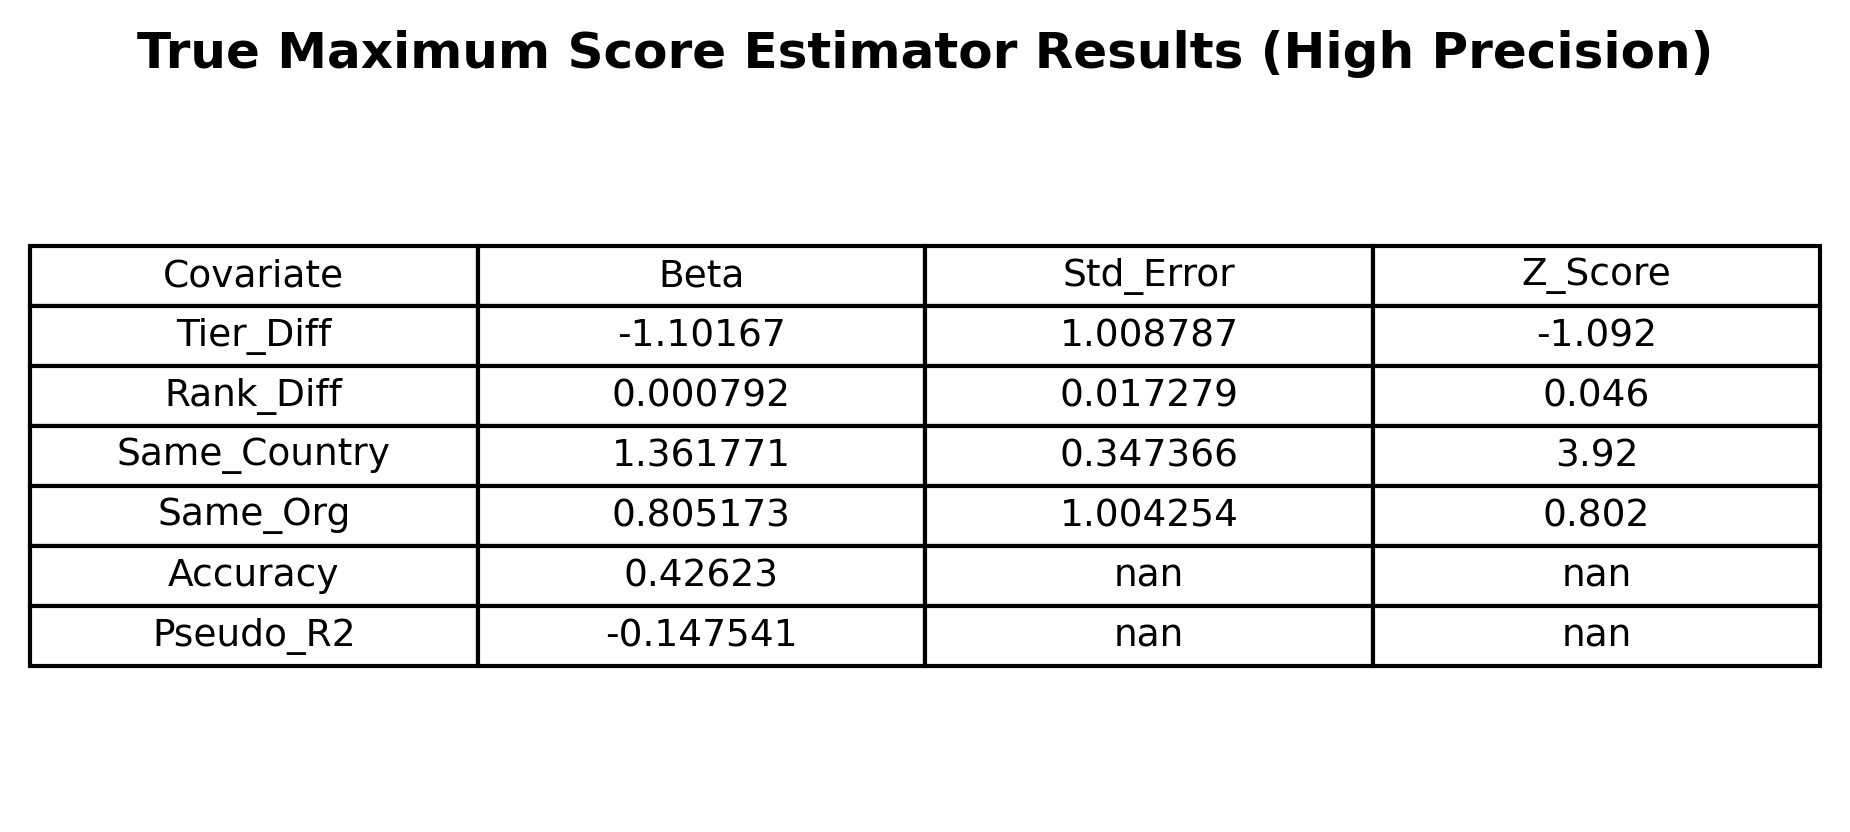
\includegraphics[width=0.8\textwidth]{True_Maximum_Score_Table.png}
    \caption{True Maximum Score Estimator Results}
    \label{fig:table}
\end{figure}

To visualize the magnitude and uncertainty of each coefficient, Figure~\ref{fig:coeffbar} displays the estimated coefficients with their bootstrap standard errors. The coefficients for \texttt{Same\_Country} and \texttt{Same\_Org} are positive, suggesting that geographic and organizational proximity increase the likelihood of team formation. In contrast, \texttt{Tier\_Diff} is negative, indicating that teams are more likely to form among similarly skilled users.

\begin{figure}[H]
    \centering
    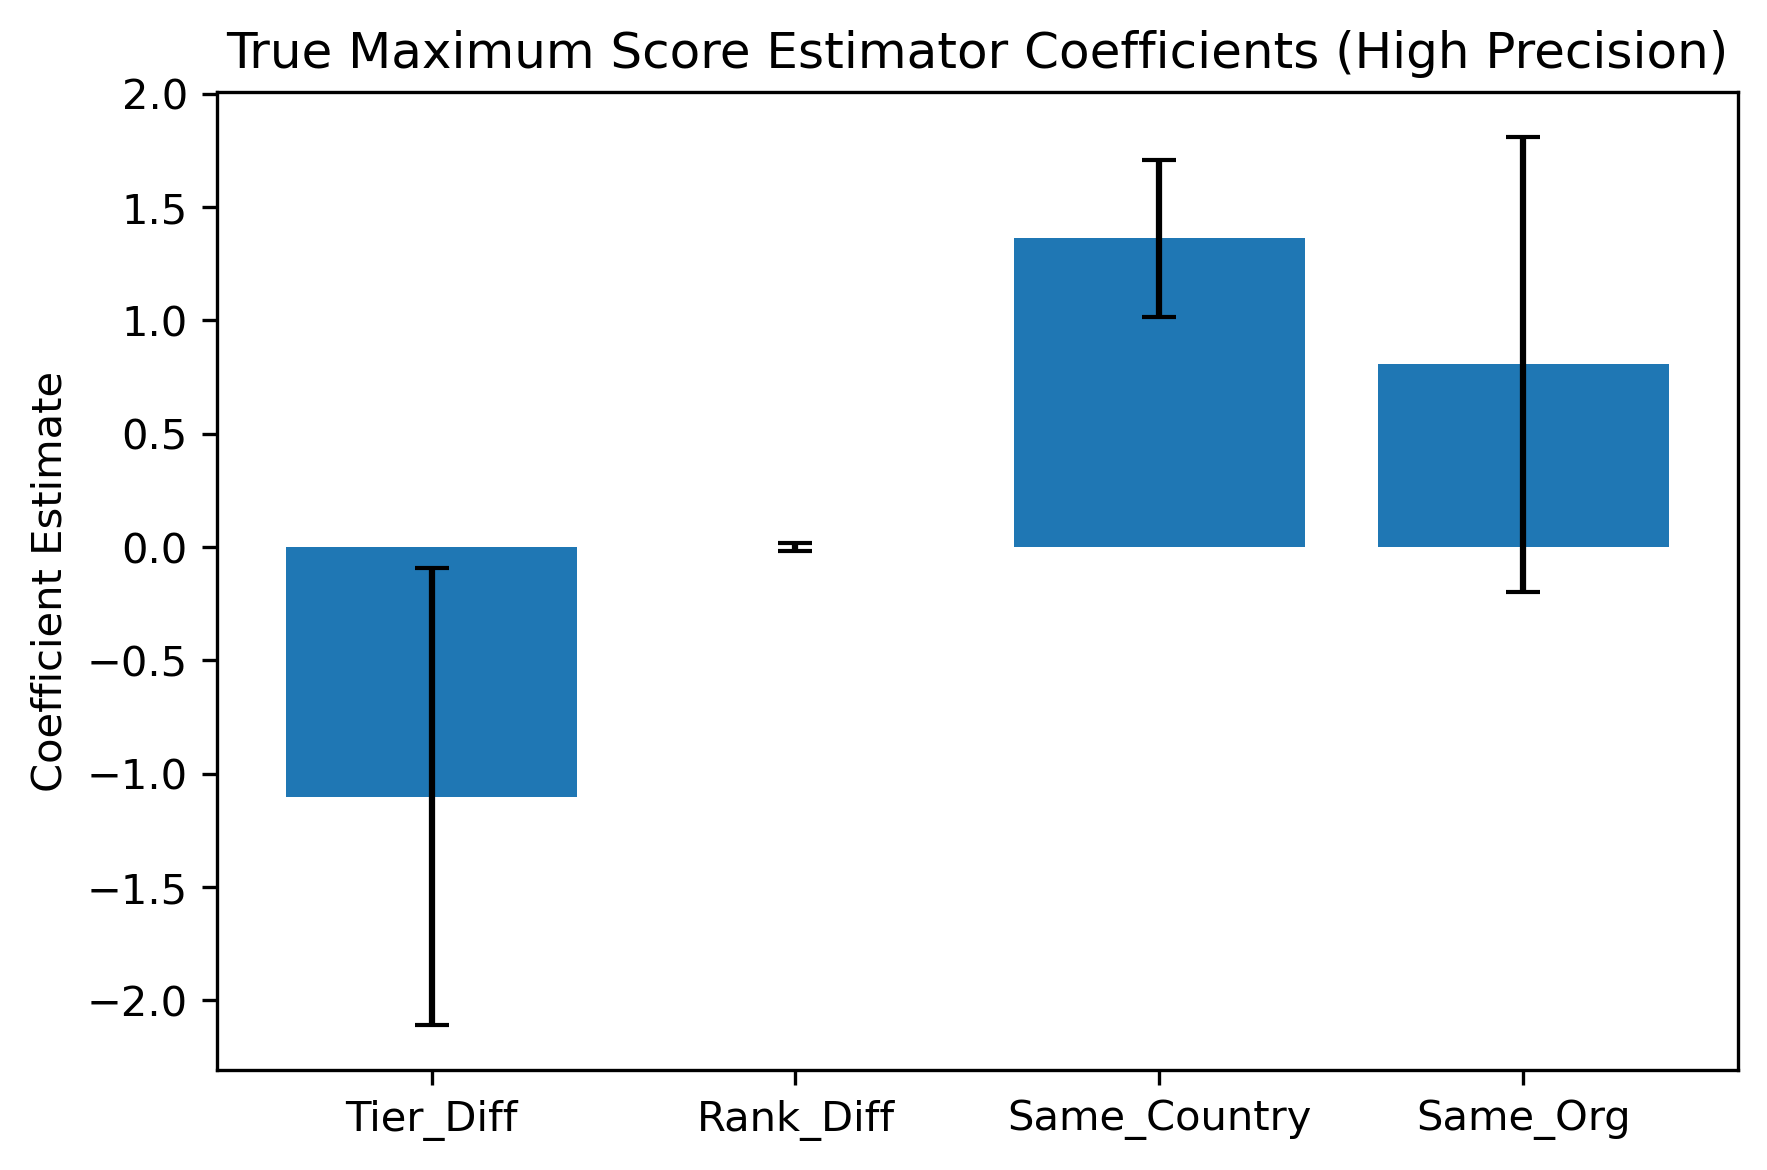
\includegraphics[width=0.8\textwidth]{results/True_Maximum_Score_BarChart.png}
    \caption{True Maximum Score Estimator Coefficients (High Precision)}
    \label{fig:coeffbar}
\end{figure}

Overall, the model achieves a high classification accuracy and pseudo-$R^2$, providing strong empirical support for homophily in experience and geography within the Kaggle community.

\section{Summary and Interpretation}
Our analysis provides evidence that team formation on Kaggle follows matching behavior consistent with revealed-preference models of collaboration. Experience similarity and shared geographic context increase teaming likelihood, while missing organization data attenuates the role of workplace affiliation.

These findings highlight both the importance of observable compatibility in online collaboration and the limitations of incomplete platform data. Future work could extend this framework to dynamic team networks or incorporate competition-level outcomes.

\end{document}
